\documentclass[twocolumn,fleqn,oneside,openany,a5paper,12pt]{book}
\usepackage{hyperref}
\usepackage{wrapfig}
\usepackage{polyglossia}
\setdefaultlanguage{polish}
%\setotherlanguage{french}
%\begin{french}
%\textsc{url:} www. \\
%\end{french}


\pagestyle{empty}
\usepackage{longtable}\usepackage{multirow} \usepackage{luacode} 
\usepackage[table]{xcolor}
\usepackage{graphicx}
\usepackage[left=2mm,right=3mm, top=1mm,bottom=5.0mm,marginparwidth=1mm, foot=.2cm,paperwidth=99mm, paperheight=132mm ]{geometry}


\usepackage{fontspec}
%\setmainfont{DejaVu Sans} 
%\setmainfont{Arial}
\setmainfont{Times  New Roman}
%\setmainfont[BoldItalicFont={Times New Roman}]{DejaVu Sans}
%\setmainfont[BoldItalicFont={Times New Roman Bold Italic}]{DejaVu Sans}

%\usepackage{draftwatermark}
%\SetWatermarkText{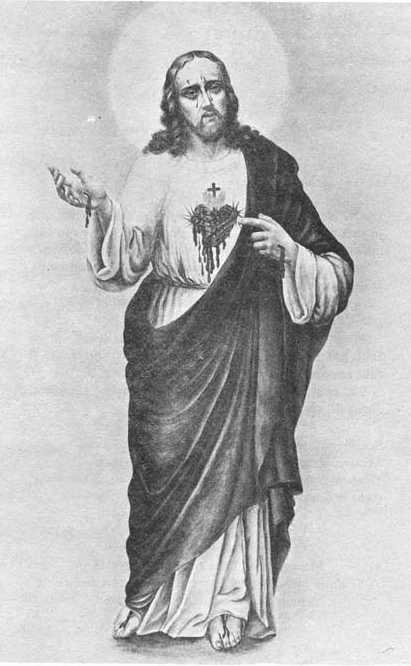
\includegraphics[width=.5\textwidth,angle=-45]{NSJ.jpg}}
%\SetWatermarkScale{1}


\def\mysec#1{\subsubsection*{#1}\addcontentsline{toc}{chapter}{#1}}

\begin{document}
\mysec{9:00 Przybądź Duchu Św.}
\begin{picture}(0,0)
\put(40,-0){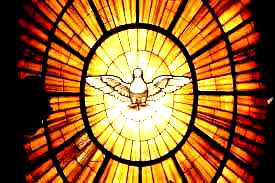
\includegraphics[width=.13\textwidth]{duchsw.jpg}}
\end{picture}
\noindent
{\obeycr\small
1. Przybądź, Duchu Św.,
Ześlij z nieba wzięty
Światła Twego strumień.
Przyjdź, Ojcze ubogich,
Przyjdź, Dawco łask drogich,
Przyjdź, światłości sumień.
2. O najmilszy z gości,
Słodka serc radości,
Słodkie orzeźwienie!
W pracy Tyś ochłodą,
W skwarze żywą wodą,
W płaczu utulenie.
3. Światłości najświętsza,
Serc wierzących wnętrza
Poddaj Twej potędze.
Bez Twojego tchnienia
Cóż jest wśród stworzenia?
Tylko cierń i nędze.
4. Obmyj, co nieświęte,
Oschłym wlej zachętę,
Ulecz serca ranę!
Nagnij, co jest harde,
Rozgrzej serca twarde,
Prowadź zabłąkane.
5. Daj Twoim wierzącym,
W Tobie ufającym,
Siedmiorakie dary!
Daj zasługę męstwa,
Daj wieniec zwycięstwa,
Daj szczęście bez miary!
}
\mysec{6:00,12:00,18:00 Anioł~Pański zwiastował}
Pannie Maryi i poczęła z Ducha Św.

{\small Módlmy się: Łaskę Twoją, prosimy Cię, Panie, racz wlać w serca nasze, abyśmy, którzy za zwiastowaniem anielskim Wcielenie Chrystusa, Syna Twego poznali, przez mękę Jego i~krzyż do chwały zmartwychwstania byli doprowadzeni. Przez Chrystusa, Pana naszego. Amen.}
\onecolumn
\mysec{Koronka do Ducha Św.}
\begin{picture}(0,0)
\put(133,7){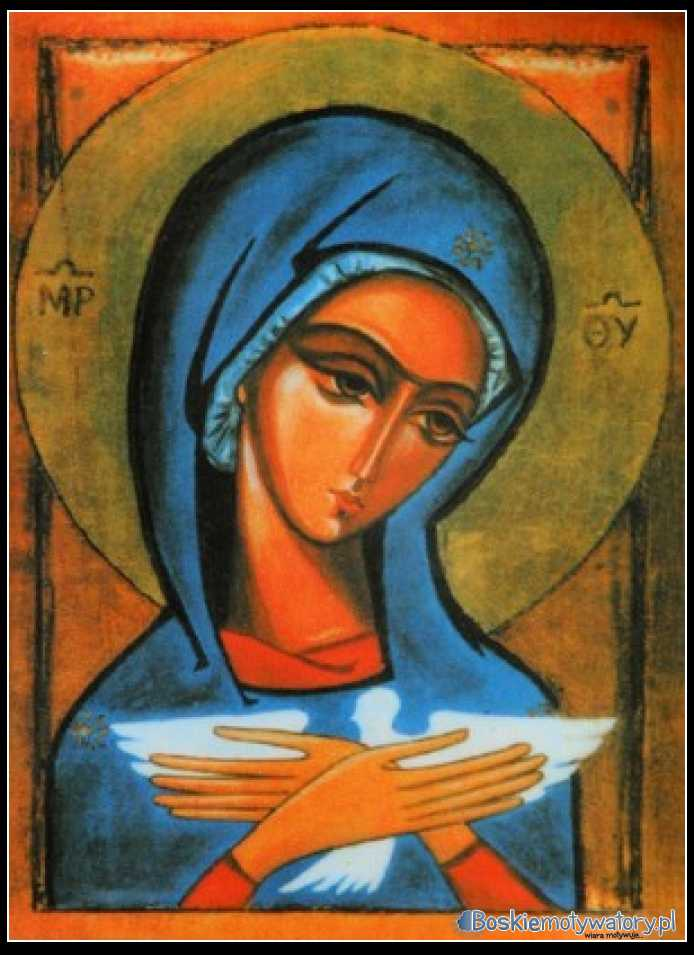
\includegraphics[width=7.5ex]{MNODS.jpg}}
\end{picture}
{\scriptsize Odmawia się jak zwykły różaniec. Po każdym dziesiątku: Chwała Ojcu..., O~Maryjo,  Niepokalana Oblubienico Ducha Świętego, módl się za nami. W~Zdrowaś Maryjo dodaje się po słowie <<Jezus>> następujące słowa (odpowiednio w każdym dziesiątku różańca):}

\noindent1. \emph{który niech usposobi nasze serca} na przyjęcie pełni łask Ducha~Św., {\tiny Święta Maryjo, Matko Boża, módl się za nami grzesznymi...}

\noindent 2. \emph{który niech nam udzieli Ducha~Św.,} pomnoży i~umocni  w~nas wiarę, nadzieję i~miłość, {\tiny Święta Maryjo...}

\noindent3. \emph{który niech nas, przez Ducha~Św.}: umocni, oświeci, prowadzi, rządzi i~uświęci, {\tiny Święta Maryjo...}

\noindent4. \emph{który niech nasze serca zapali miłością Ducha~Św.} i~napełnia najgłębszą pokorą, łagodnością, cierpliwością, uległością, oddaniem, mocą i świętością, {\tiny Święta Maryjo...}

\noindent5. \emph{który niech ześle nam 7 darów oraz owoce Ducha~Św.} i użycza wszystkiego, co dobre, a powstrzymuje od wszystkiego, co złe, {\tiny Święta Maryjo...}

\vbox{
\noindent{\bf\tiny OFIAROWANIE}

Ojcze Przedwieczny, ofiaruję Ci drogocenną Krew Chrystusa --- przez Najświętsze Serce Pana Jezusa i Najświętszej Maryi Panny --- na otrzymanie darów Ducha Świętego dla ratowania dusz. Amen. 

Ojcze Niebieski, ofiaruję Ci przez Matkę Najświętszą --- nieskończoną ilość razy, przez całą wieczność, w imieniu wszystkich i za wszystkie dusze --- Miłość Ducha Świętego, ze wszystkimi jej skutkami w życiu doczesnym i wiecznym. Amen.}

\twocolumn
\mysec{Modlitwa o świętość kapłanów (św. Faustyna)}
O Jezu mój, proszę Cię za Kościół cały, udziel mu miłości i światła Ducha Swego. 

Daj moc słowom kapłańskim, aby serca zatwardziałe kruszyły się i wróciły do Ciebie Panie.

Panie daj nam świętych kapłanów, Ty Sam ich utrzymuj w świętości. 
 
O Boski i Najwyższy Kapłanie, niech moc miłosierdzia Twego towarzyszy im wszędzie i chroni ich od zasadzek i
sideł diabelskich, które ustawicznie zastawia na dusze kapłana.

Niechaj moc miłosierdzia Twego o Panie, kruszy i wniwecz obraca wszystko to co by mogło przyćmić świętość kapłan,
bo Ty wszystko możesz.(Dz 1052)

\mysec{Litania do Ducha Św.}
{\obeycr
Chwała Ojcu i Synowi i Duchowi Świętemu …

1. Duchu Święty, zstąp z tronu Twojej chwały i rozbij swój  namiot w sercach sług twoich {\tiny Bądź pochwalony}
2. Duchu Święty, który od Ojca i Syna pochodzisz, ucz  mnie żyć w stałej obecności Bożej {\tiny Bądź pochwalony}
3. Duchu Święty, który od Ojca i Syna pochodzisz, ucz mnie żyć zgodnie z wolą Najwyższego {\tiny Bądź pochwalony}
4. Duchu Święty, który mieszkasz w sercach synów Bożych, pouczaj mnie, bym mógł Ciebie poznać i prawdziwie pokochać {\tiny Bądź pochwalony}
5. Duchu Święty, który troszczysz się o Chwałę Ojca,  ucz mnie żyć w całkowitym oddaniu i zawierzeniu Bogu {\tiny Bądź pochwalony}
6. Duchu Święty, w znaku języków ognistych, zapal w moim sercu ogień Twej miłości {\tiny Bądź pochwalony}
7. Duchu Święty, tajemnicza Gołębico, ucz mnie dobrze zrozumieć Pismo Święte {\tiny Bądź pochwalony}
8. Duchu Święty, który nie masz ani oblicza ani imienia,  naucz mnie dobrze modlić się {\tiny Bądź pochwalony}
9. Duchu Święty, który przemawiasz przez usta proroków, naucz mnie żyć w równowadze ducha i zachować pokój serca  {\tiny Bądź pochwalony}
10. Duchu Święty, gorejące ognisko miłości,  ucz mnie mądrości życia oraz cierpliwości {\tiny Bądź pochwalony}
11. Duchu Święty, Dawco wszelkich darów,  ucz mnie żyć w pokorze i skromności {\tiny Bądź pochwalony}
12. Duchu Święty, przeobfita skarbnico łask, ucz mnie pojmować wartość cierpienia {\tiny Bądź pochwalony}
13. Duchu Święty, bezdenna skarbnico łask, ucz mnie dobrze wykorzystać cenny czas {\tiny Bądź pochwalony}
14. Duchu Święty, niewyczerpana skarbnico łask, broń mnie przed jakimkolwiek brakiem miłości i przed pychą {\tiny Bądź pochwalony}
15. Duchu Święty, którego bogactwa nikt ogarnąć nie zdoła, ucz mnie odrzucać bezużyteczne wyobrażenia i myśli {\tiny Bądź pochwalony}
16. Duchu Święty, Dawco wielu darów, ucz mnie rezygnować z bezużytecznych działań i unikać niepotrzebnych rozmów {\tiny Bądź pochwalony}
17. Duchu Święty, z którego pełni wszyscyśmy otrzymali, ucz mnie milczenia i mówienia we właściwym czasie {\tiny Bądź pochwalony}
18. Duchu Święty, wieczysta miłości,  ucz mnie dawać innym dobry przykład {\tiny Bądź pochwalony}
19. Duchu Święty, wieczysta Dobroci, daj mi wytrwanie w dobrym {\tiny Bądź pochwalony}
20. Duchu Święty, słodki Nauczycielu, naucz mnie w sposób właściwy obchodzić się z ludźmi {\tiny Bądź pochwalony}
21. Duchu Święty, najmilszy przyjacielu dusz, ucz mnie nikogo nie sądzić i doznanych krzywd nie pamiętać {\tiny Bądź pochwalony}
22. Duchu Święty, uszczęśliwiające światło duszy, tak mnie prowadź, bym widział potrzeby innych i nie zaniedbywał dobrych dzieł {\tiny Bądź pochwalony}
23. Duchu Święty, Ojcze ubogich, daj bym poznał swoje błędy {\tiny Bądź pochwalony}
24. Duchu Święty, który w duszach dokonujesz swych cudów, ucz mnie czuwać nad sobą i prowadź do doskonałości {\tiny Bądź pochwalony}
25. Duchu Święty, przed którym nic nie jest zakryte,  ucz mnie, jak unikać podstępu złego ducha {\tiny Bądź pochwalony}
26. Duchu Święty, który znasz przyszłość wszechświata, pomóż mi uwolnić się spod władania ciała i szatana {\tiny Bądź pochwalony}
27. Duchu Święty, który znasz także moją przyszłość, Twojej opiece powierzam moją rodzinę, przyjaciół, dobroczyńców i wszystkich ludzi {\tiny Bądź pochwalony}
28. Duchu Święty, dzięki Twej Boskiej pomocy, nauczaj mnie żyć dla chwały Bożej, dla zbawienia dusz i ku czci Matki Bożej, abym mógł umierać jako wierny sługa {\tiny Bądź pochwalony} 
}

{\tiny Jam Jest Duch Święty, Trzecia Osoba Trójcy Świętej. Słuchaj człowiecze Moich Słów, słuchaj uważnie. Dziś pragnę poprosić was Moje stworzenia, abyście zaczęli Mnie czcić w sposób szczególny. Pragnę, aby obchodzono każdego 3 dnia miesiąca, dzień przeznaczony ku czci Ducha Świętego. Głównym świętem nadal pozostaje Święto Zesłania Ducha Świętego. Ponadto proszę, aby każdy kto tylko zdoła, a obowiązku stanu pozwolą, niech się pomodli do Mojej Osoby - Ducha Świętego o 9:00 rano. Gdy jest to niemożliwe, aby się pomodlić, wystarczy choćby krótkie westchnienie. Obiecuję wszystkim, którzy czcić Mnie będą, szczególne Moje Łaski i Dary oraz Moją opiekę nad tą duszą oraz nad całą rodziną. Daruję przewinienia przodków karane do czwartego pokolenia. Pragnę, aby dusza wasza, przygotowała się do każdego święta Nowenną i Koronką do Ducha Świętego. }


\mysec{Litania Loretańska do Najświętszej Maryi Panny...}
\textbf{Módlmy się.} Panie, nasz Boże, daj nam, sługom swoim, cieszyć się trwałym zdrowiem duszy i~ciała, † i~za wstawiennictwem Najświętszej Maryi, zawsze Dziewicy, * uwolnij nas od doczesnych utrapień i~obdarz wieczną radością. Przez Chrystusa, Pana naszego. Amen.

\newpage
\mysec{Nowenna do Matki Bożej Nieustającej Pomocy}
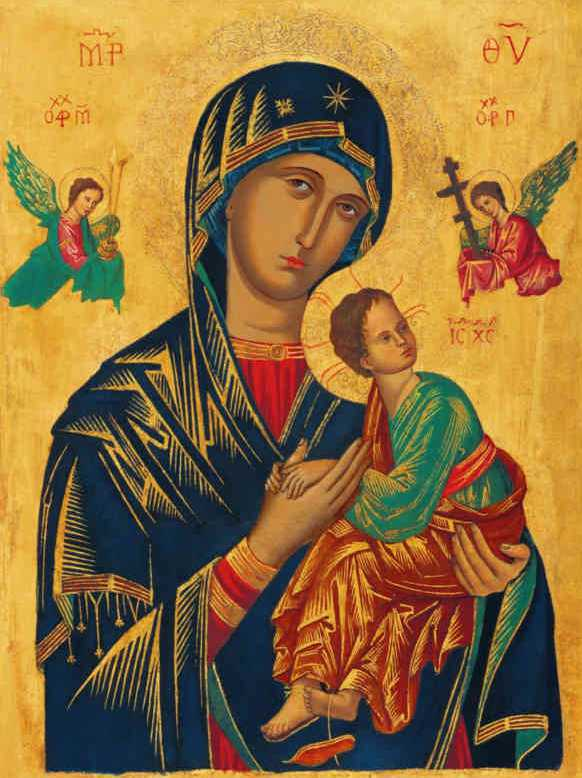
\includegraphics[width=.4\textwidth]{MatkaBNP.jpg}
O~Matko Nieustającej Pomocy, z największą ufnością przychodzę dzisiaj przed Twój święty obraz, by błagać o pomoc Twoją. Nie liczę na moje zasługi, ani na moje dobre uczynki, ale tylko na nieskończone zasługi Pana Jezusa i na Twoją niezrównaną miłość macierzyńską. Tyś patrzyła, o Matko, na rany Odkupiciela i na krew Jego wylaną na krzyżu dla naszego zbawienia. Tenże Syn Twój umierając, dał nam Ciebie za Matkę. Czyż więc nie będziesz dla nas, jak głosi Twój słodki tytuł: Nieustającą Wspomożycielką? Ciebie więc, o Matko Nieustającej Pomocy, przez bolesna mękę i śmierć Twego Boskiego Syna, przez niewypowiedziane cierpienia Twego Syna, o Współodkupicielko, błagam najgoręcej, abyś wyprosiła mi u Syna Twego tę łaskę, której tak bardzo pragnę i tak bardzo potrzebuję {\footnotesize (przedstaw Matce Bożej twoje prośby)}.

Ty wiesz, o Matko Przebłogosławiona, jak bardzo Jezus, Odkupiciel nasz, pragnie udzielić nam wszystkich owoców Odkupienia. Ty wiesz, że skarby te zostały złożone w Twoje ręce, abyś je nam rozdzielała. Wyjednaj mi przeto, o Najłaskawsza Matko, u Serca Jezusowego tę łaskę, o którą w tej nowennie pokornie proszę, a ja z radością wychwalać będę Twoje miłosierdzie przez całą wieczność. Amen.

\mysec{Akt oddania się Niepokalanej} 
\begin{wrapfigure}{l}{1cm}

\includegraphics[width=1cm]{niepokalana.jpg}
\end{wrapfigure}
O~Niepokalana, nieba i~ziemi Królowo, Ucieczko grzesznych i~Matko nasza najmiłościwsza.

Ty, której Bóg cały porządek miłosierdzia powierzyć raczył.

Ja, niegodny grzesznik, rzucam się do stóp Twoich, kornie błagając, abyś mnie całego i~zupełnie za rzecz i~własność swoją przyjąć raczyła i~uczyniła ze mną, wraz ze wszystkimi władzami mej duszy i~ciała, i~z~całym mym życiem, śmiercią i~wiecznością, cokolwiek Ci się podoba.

Użyj także, jeżeli zechcesz, mnie całego, bez żadnego zastrzeżenia, do dokonania tego, co o~Tobie powiedziano: ,,Ona zetrze głowę twoją", jako też: "Wszystkie herezje samaś zniszczyła na całym świecie", abym w Twoich niepokalanych i~najmiłościwszych rękach stał się użytecznym narzędziem do zaszczepienia i~jak najsilniejszego wzrostu Twej chwały w tylu zbłąkanych i~obojętnych duszach, a~w ten sposób do jak największego rozszerzenia błogiego Królestwa Najświętszego Serca Jezusowego: albowiem gdzie Ty wejdziesz, tam łaskę nawrócenia i~uświęcenia wypraszasz, przez Twoje bowiem ręce wszelkie łaski z~Najsłodszego Serca Jezusowego na nas spływają.

Dozwól mi chwalić Cię, Panno Przenajświętsza.

Daj mi moc przeciw nieprzyjaciołom Twoim.
\vfill
\mysec{Litania do Najświętszego Serca Pana Jezusa}
\begin{picture}(0,0)
\put(40,-135){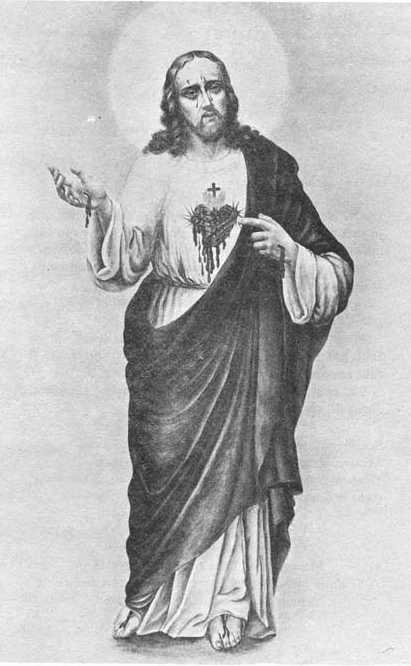
\includegraphics[width=.3\textwidth]{NSJ.jpg}}
\end{picture}
\def\spojnik#1{{\tiny #1}}
\def\sji#1{
\includegraphics[height=1ex]{sj.pdf}{\tiny #1}}
\def\sj{{\tiny $\rm Serce \atop Jezusa$}}
\begingroup\obeycr
Kyrie, eleison(...)
\sj Syna O~p
\sj w łonie M-D p D Ś u
\sj ze Słowem B i z

\sj nieskończonego m
\sj świątynio B
\sj przybytku N
\sj domie Boży \spojnik{i} b n
\sji 8
\sj gorejące o~m
\sj sprawiedliwości \spojnik{i} m s
\sj dobroci \spojnik{i} m p

\sj cnót w b g
\sj wszelkiej ch n
\sj królu \spojnik{i} z~s w
\sji {14}
\sj w którym~są~w~s~m~\spojnik{i}~u
\sj w którym m c p b
\sj w którym s O~b u~
\sj z~którego p w o
\sji {18}
\sj odwieczne u~ś
\sj cierpliwe \spojnik{i} w m
\sj hojne d w, k C w
\sj źródło ż \spojnik{i} ś
\sj przebłaganie z~g n
\sji {23}
\sj zelżywością n
\sj dla n n s
\sj aż d ś p
\sji {26}
\sj włócznią p
\sj źródło w p
\sj życie \spojnik{i} z~n
\sji {29}
\sj pokoju \spojnik{i} p n
\sj krwawa o~g
\sj zbawienie u~w T
\sj nadziejo w T~u
\sj rozkoszy w ś
 
{\tiny Baranku Boży... 
K. Jezu cichy i~pokornego Serca.
W. Uczyń serca nasze według Serca Twego.}
\endgroup 
Módlmy się\\
Wszechmogący, wieczny Boże, wejrzyj na serce najmilszego Syna Swego i~na chwałę, i~zadośćuczynienie, jakie w imieniu grzeszników Ci składa. 
Daj się przebłagać tym, którzy żebrzą Twego miłosierdzia i~racz udzielić przebaczenia w imię tegoż Syna Swego, Jezusa Chrystusa, który z~Tobą żyje i~króluje na wieki wieków. Amen.
 
\subsubsection*{Akt poświęcenia całego rodzaju ludzkiego Sercu Jezusowemu}
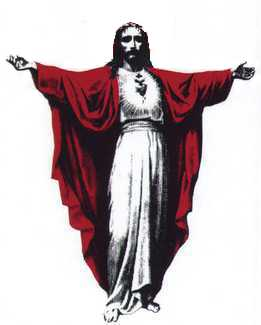
\includegraphics[width=.4\textwidth]{SerceJezusa.jpg}\\
K. O~Jezu Najsłodszy, Odkupicielu rodzaju ludzkiego, wejrzyj na nas, korzących się u~stóp Twego ołtarza.

W. Twoją jesteśmy własnością i~do Ciebie należeć chcemy.

K. Oto dzisiaj każdy z~nas oddaje się dobrowolnie Najświętszemu Sercu Twemu, aby jeszcze ściślej zjednoczyć się z~Tobą. Wielu nie zna Ciebie wcale, wielu odwróciło się od Ciebie, wzgardziwszy przykazaniami Twymi. Zlituj się nad jednymi i~drugimi, o~Jezu najłaskawszy, i~pociągnij wszystkich do świętego Serca swego.

Królem bądź nam, o~Panie, nie tylko wiernym, którzy nigdy nie odstąpili od Ciebie, ale i~synom marnotrawnym, którzy Cię opuścili.

W. Spraw, aby do domu rodzicielskiego wrócili co prędzej i~nie zginęli z~nędzy i~głodu.

K. Króluj tym, których albo błędne mniemania uwiodły, albo niezgoda oddziela: przywiedź ich do przystani prawdy i~jedności wiary, aby rychło nastała jedna owczarnia i~jeden pasterz. Użycz Kościołowi Twemu bezpiecznej wolności. Udziel wszystkim narodom spokoju i~ładu. Spraw, aby ze wszystkiej ziemi, od końca do końca jeden brzmiał głos:

W. Chwała bądź Bożemu Sercu, przez które stało się nam zbawienie. Jemu cześć i~chwała na wieki. Amen.\vfill



\mysec{Litania do św. Józefa ...}
\begin{center}
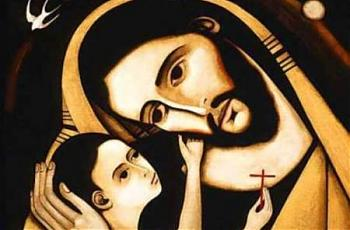
\includegraphics[width=.4\textwidth]{swJozef.jpg}
\end{center}
Módlmy się:
Boże, Ty w niewysłowionej Opatrzności wybrałeś świętego Józefa na Oblubieńca Najświętszej Rodzicielki Twojego Syna, spraw, abyśmy oddając Mu na ziemi cześć jako Opiekunowi, zasłużyli na jego orędownictwo w niebie. Przez Chrystusa, Pana naszego. Amen.
\newpage
\paragraph{Modlitwa papieża Leona XIII}
Do Ciebie, święty Józefie, uciekamy się w naszej niedoli. Wezwawszy pomocy Twej Najświętszej Oblubienicy z~ufnością również błagamy o~Twoją opiekę. Przez miłość, która Cię łączyła z~Niepokalaną Dziewicą Bogarodzicą i~przez ojcowską Twą troskliwość, którą otaczałeś Dziecię Jezus, pokornie błagamy: wejrzyj łaskawie na dziedzictwo, które Jezus Chrystus nabył Krwią swoją i~swoim potężnym wstawiennictwem dopomóż nam w naszych potrzebach. 

Opatrznościowy Stróżu Bożej Rodziny, czuwaj nad wybranym potomstwem Jezusa Chrystusa. Oddal od nas, ukochany Ojcze, wszelką zarazę błędów i~zepsucia. Potężny nasz Wybawco, przybądź nam łaskawie z~niebiańską pomocą w tej walce z~mocami ciemności. A~jak niegdyś uratowałeś Dziecię Jezus z~niebezpieczeństwa, które groziło Jego życiu, tak teraz broń świętego Kościoła Bożego od wrogich zasadzek i~od wszelkich przeciwności. 

Otaczaj każdego z~nas nieustanną opieką, abyśmy za Twoim przykładem i~Twoją pomocą wsparci mogli żyć świątobliwie, umrzeć pobożnie i~osiągnąć wieczną szczęśliwość w niebie. Amen.\vfill

\subsubsection*{Modlitwa do św. Michała Archanioła}
Święty Michale Archaniele, wspomagaj nas w walce, a~przeciw niegodziwości i~zasadzkom złego ducha bądź naszą obroną. Oby go Bóg pogromić raczył, pokornie o~to prosimy, a~Ty, Wodzu niebieskich zastępów, szatana i~inne duchy złe, które na zgubę dusz ludzkich po tym świecie krążą, mocą Bożą strąć do piekła. Amen.
\begin{center}
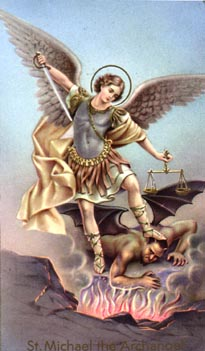
\includegraphics[width=2cm]{michalArchaniol.jpg}
\end{center}

\vfill



\newpage
\mysec{Modlitwa podyktowana św. Gertrudzie}
\def\ref{ Amen. \mbox{{\tiny\raisebox{.2ex}{\textbf{O}} Z \raisebox{.2ex} {\textbf{J}}}}}
\ref\ = (Ojcze nasz, Zdrowaś Maryjo, Westchnienie: Jezu, Miłości moja, bądź uwielbiony i~zmiłuj się nade mną grzesznym.)
 

\noindent\textbf{1.} \textsc{\footnotesize  O~Jezu Chryste! Słodkości odwieczna wszystkich, obejmujących Cię miłością}, Radości przewyższająca wszelkie szczęście i~oczekiwanie, prawdziwe Zbawienie i~Nadziejo każdego grzesznika. Ty, który objawiłeś, że największym Twoim zadowoleniem jest być między ludźmi, tak że z~miłości dla nich po upływie zapowiedzianych czasów przyjąłeś naturę ludzką.

Wspomnij sobie, o~Jezu, wszystkie cierpienia zniesione od chwili poczęcia, a~zwłaszcza w czasie swojej świętej Męki, jak to przewidziała myśl Boża i~jak zdecydowała wola Najwyższego. 

Wspomnij sobie, Panie, że urządzając Wieczerzę Eucharystyczną wraz z~uczniami, po umyciu nóg, dałeś swoje Najświętsze Ciało i~drogocenną Krew, a~udzielając pociechy z~właściwą sobie dobrocią przepowiedziałeś bliską swoją Mękę. 

Wspomnij na smutek i~gorycz, które w udręczonej duszy odczułeś, wyznając wobec najbliższego otoczenia: „Smutna jest dusza moja aż do śmierci”. 

Wspomnij wszystkie obawy, niepokoje i~boleści, które Twoje delikatne ciało znosiło przed ukrzyżowaniem, kiedy po odprawieniu po raz trzeci modlitwy, oblewając się krwawym Potem, zostałeś zdradzony przez swojego ucznia Judasza, aresztowany przez wybrany naród, oskarżony przez fałszywych świadków, niesprawiedliwie sądzony przez trzech sędziów, tuż przed uroczystym świętem Wielkanocy czyli Paschy. 

Wspomnij, że przywiązano Cię do słupa i~rozdarto Ciało biczami, że byłeś obnażony z~własnych szat i~odziany w inny strój na pośmiewisko, że Cię ukoronowano cierniami, do ręki włożono trzcinę, zasłonięto oczy i~twarz, że Cię policzkowano i~obrzucono obelgami. 

Na pamiątkę tych wszystkich zniewag i~boleści, które wycierpiałeś w okresie poprzedzającym Mękę Krzyża, daj mi przed nadejściem śmierci przeżyć prawdziwą skruchę serca, szczerą i~całkowitą spowiedź, odprawić godne zadośćuczynienie i~otrzymać odpuszczenie wszystkich grzechów.\ref
	
\noindent\textbf{2.} \textsc{\footnotesize O~Jezu! Prawdziwa wolności Aniołów, Raju niezmąconego szczęścia}, wspomnij sobie na odrazę i~smutek, które odczułeś, kiedy nieprzyjaciele otoczyli Cię jak wściekłe lwy i~tysiącami zniewag, policzkowaniem, kaleczeniem, i~innymi wymyślnymi udrękami prześcigali się w zadawaniu cierpień. Ze względu na te tortury i~stek obelżywości, błagam Cię, Boski Zbawicielu, wyzwól mnie z~więzów wszystkich nieprzyjaciół widzialnych i~niewidzialnych, a~roztaczając błogosławioną opiekę prowadź drogą doskonałości do zbawienia wiecznego.\ref
	
\noindent\textbf{3.} \textsc{\footnotesize O~Jezu! Stworzycielu nieba i~ziemi}, którego żadna rzecz nie może ograniczyć ani objąć. Ty, który ogarniasz i~zespalasz wszystko swoją potęgą, wspomnij sobie na gorzką boleść, którą odczuwałeś, kiedy kaci, przywiązują Twoje święte ręce i~nogi do krzyża, przeszyli je na wylot grubymi, stępionymi gwoździami. Rozciągając Cię z~niesłychanym okrucieństwem na krzyżu, nie syci Twych cierpień, miotali obelgi na wszystkie strony i~dając upust swojej wściekłości, powiększali Twoje Rany przez zadawanie dodatkowych katuszy. 

Ze względu na ogrom cierpień, których doświadczyłeś podczas ukrzyżowania, daj mi Twoją świętą bojaźń i~Twoją prawdziwą miłość.\ref
	
\noindent\textbf{4.} \textsc{\footnotesize O~Jezu! Lekarzu niebieski}, wzniesiony na krzyżu, by nasze rany uleczyć Twoimi, wspomnij na obicia i~złamania, jakich doznałeś w swoich członkach, tak że każdy z~nich został w jakiś sposób naruszony. Od stóp do głów nie znaleziono miejsca na Twoim Ciele, które nie byłoby pokryte raną. W takim stanie poniżenia, zapominając o~własnych cierpieniach, nie przestawałeś modlić się do Ojca za nieprzyjaciół słowami: „Ojcze, odpuść im, bo nie wiedzą co czynią”! 

Na mocy twego bezgranicznego Miłosierdzia i~na pamiątkę owej boleści, spraw, żeby pamięć o~Twojej gorzkiej Męce przywiodła nas do doskonałej skruchy i~przyniosła odpuszczenie wszystkich grzechów.\ref
	
\noindent\textbf{5.} \textsc{\footnotesize O~Jezu! Zwierciadło odwiecznego Blasku}, wspomnij na smutek, którego doznałeś, kiedy w świetle Boskiego poznania, rozważając nad przeznaczeniem tych, którzy mieli być odkupieni dzięki zasługom Twojej świętej Męki, widziałeś zarazem wielkie tłumy skazanych, którzy szli na potępienie z~powodu rozlicznych grzechów. Żal Ci było tych nieszczęśliwych ludzi zgubionych i~zrozpaczonych. 

Przez to bezgraniczne współczucie i~miłosierdzie, a~zwłaszcza przez wzruszającą dobroć okazaną skruszonemu łotrowi współ\-u\-krzyż\-owa\-ne\-mu  na Golgocie, kiedy Mu powiedziałeś: „Dziś ze Mną będziesz w raju!”, błagam Cię, o~słodki Jezu, okaż miłosierdzie mnie grzesznemu w godzinę śmierci.\ref
	
\noindent\textbf{6.} \textsc{\footnotesize O~Jezu! Łaskawy i~upragniony Królu}, wspomnij na boleść, którą odczułeś, kiedy nagi jak nędzarz, przykuty do krzyża, zostałeś na tym drzewie hańby wyśmiany i~wzgardzony. Wszyscy Twoi krewni i~przyjaciele opuścili Cię z~wyjątkiem ukochanej Matki, która stała wiernie przy tobie podczas konania. Ty zaś poleciłeś Ją swojemu wiernemu Uczniowi, mówiąc do Najświętszej Maryi Panny: „Niewiasto, oto syn Twój!” i~do świętego Jana: „Oto Matka Twoja!”

Błagam Cię, o~mój Zbawicielu, przez miecz boleści, który ongiś przeszył duszę Twojej Najboleśniejszej Matki, współczuj ze mną we wszystkich utrapieniach i~doświadczeniach, zarówno cielesnych jak i~duchowych, abym je wszystkie przezwyciężył w życiu a~zwłaszcza w ostatniej godzinie przed nadejściem śmierci.\ref
	
\noindent\textbf{7.} \textsc{\footnotesize O~Jezu! Źródło niewyczerpalnej litości}, który z~głęboką miłością wypowiedziałeś na krzyżu tęsknotę: „Pragnę!” Było to pragnienie zbawienia rodzaju ludzkiego. Proszę Cię, o~mój Odkupicielu, rozpal pragnienia naszych serc, byśmy wytrwale we wszystkich podejmowanych czynnościach dążyli do doskonałości. Wygaś w nas całkowicie pożądliwość ciała i~żądze światowe.\ref
	
\noindent\textbf{8.} \textsc{\footnotesize O~Jezu! Słodyczy serc, niepojęta Dobroci}, przez gorzką żółć i~ocet, których skosztowałeś na krzyżu z~miłości ku nam, spraw, byśmy godnie przyjmowali Twoje Ciało i~Twoją bezcenną Krew, lekarstwo i~pociechę naszych dusz, w czasie ziemskiego pielgrzymowania i~w godzinie śmierci.\ref
	
\noindent\textbf{9.} \textsc{\footnotesize O~Jezu! Cnoto królewska, Radości ducha}, wspomnij na boleść, którą znosiłeś, kiedy zatopiony w smutku z~powodu zbliżającej się śmierci, znieważony, wykpiony przez wybrany naród, opuszczony przez Ojca Twego, wołałeś głośno: „Boże Mój, Boże Mój, czemuś Mnie opuścił?” 

Zaklinam Cię, o~mój Zbawicielu, przez doznaną trwogę, abyś mnie nie opuścił podczas cierpienia i~trwogi, jakie wywołuje zbliżająca się śmierć i~sąd Boży.\ref
	
\noindent\textbf{10.} \textsc{\footnotesize O~Jezu! który jesteś Początkiem i~Końcem wszystkich rzeczy, Życiem i~Szczytem cnót}, wspomnij sobie, że ze względu na mnie zostałeś pogrążony w niezmierzonych boleściach. Przez ten bezmiar cierpień, spowodowany okrutnymi Ranami, które zadały grzechy świata, naucz mnie zachować z~prawdziwą Miłością Twoje przykazania, bo one dla tych, którzy Cię kochają, są łatwą i~jedyną drogą do zbawienia.\ref
	
\noindent\textbf{11.} \textsc{\footnotesize O~Jezu! Niezgłębione źródło Miłosierdzia}, błagam Cię z~uwagi na pamięć o~Twoich Ranach, których dojmujący ból doszedł do szpiku kości i~wypełnił wszystkie wnętrzności, wyrwij mnie nędznego z~grzechów i~ukryj w głębi Ran przed zagniewanym Obliczem Sprawiedliwości, aż minie Twe oburzenie i~słuszny gniew.\ref
	
\noindent\textbf{12.} \textsc{\footnotesize O~Jezu! Zwierciadło prawdy}, Miłości, zwieńczająca wszystkie siły ducha, Znaku jedności, rozdarty i~umęczony obfitym upływem godnej uwielbienia Krwi, wspomnij na niezliczone Rany, które okryły Cię od stóp do głów. O~niezmierna i~totalna boleści, którą znosiłeś w swym dziewiczym Ciele z~miłości ku nam. Jezu Chryste, co mogłeś nadto dla mnie uczynić? Czego jeszcze nie dokonałeś? 

Zaklinam Cię, o~mój Zbawicielu, wszystkie swoje Rany znacz drogocenną Krwią w moim sercu, abym mógł w nim ustawicznie czytać boleść i~miłość Twoją. Spraw, aby przez moje przylgnięcie do Twojej Męki zaznaczył się w mojej duszy owoc Twych cierpień. Niech Twoja miłość wzrasta w niej codziennie do czasu, aż stanę przed Tobą, Skarbie wszystkich dóbr i~wszystkich radości. O~słodki Jezu, daj mi w życiu wiecznym to, o~co Cię błagam.\ref
	
\noindent\textbf{13.} \textsc{\footnotesize O~Jezu! Odwieczna Potęgo, Królu nieśmiertelny i~niezwyciężony}, wspomnij na boleść, którą znosiłeś, kiedy opuściły Cię wszystkie siły, zarówno ciała jak i~ducha, kiedy skłaniając głowę oświadczyłeś: „Wykonało się”. Błagam Cię, Panie Jezu, przez zupełne wyczerpanie i~przygniatający niepokój, jakich doznałeś przed dopełnieniem dzieła Odkupienia, zmiłuj się nade mną w ostatniej godzinie życia, kiedy dusza moja będzie w udręce, a~serce pełne trwogi. W Tobie ufność pokładam.\ref
	
\noindent\textbf{14.} \textsc{\footnotesize O~Jezu! Jedyny Synu Ojca, Blasku i~Wyrazie Jego istoty}, wspomnij na serdeczne i~pokorne polecenie się Ojcu w ufnej wypowiedzi: „Ojcze w ręce Twoje oddaję ducha mego”. I~wtedy skonałeś. Ale choć całe Ciało okaleczone i~zbroczone Krwią, oddając ostatnie tchnienie, przestało żyć, Twa Boska moc otworzyła źródło Miłosierdzia i~wylała zdroje łask odkupieńczych dla ludzkości. 

Przez tę drogocenną śmierć i~wszystkie jej okoliczności błagam Cię, Królu Świętych, wzmocnij mnie i~pomóż w walce przeciw szatanowi, ciału i~krwi, ażebym umarły dla świata żył tylko Tobą i~dla Ciebie. Proszę gorąco, przyjmuj w godzinę śmierci moją pielgrzymią i~wygnańczą duszę u~bram wieczności.\ref

\noindent\textbf{15.}  \textsc{\footnotesize O~Jezu! Usymbolizowany w życiodajnej, rajskiej winorośli}, wspomnij na obficie broczącą Krew, która popłynęła hojnie z~Twego Ciała jak wino z~dojrzałych gron w tłoczni. 

Przebity włócznią żołnierza wylałeś wszystką Krew i~Wodę do ostatniej kropli. Wisząc wysoko na krzyżu z~opadłą Najświętszą Głową, stałeś się jak pęk zeschniętej mirry, bezwładny, odrętwiały, bez śladu życia na zewnątrz i~we wnętrzu Ciała, aż do szpiku kości. 

Przez gorzką Mękę i~przez wylaną drogocenną Krew błagam Cię, o~słodki Jezu, zrań moje serce łaską, ażeby łzy pokuty i~miłości stały się dla mnie dniem i~nocą tak potrzebne, jak chleb powszedni. Nawróć mnie całkowicie do Siebie, aby me serce utworzyło dla Ciebie stałe mieszkanie, aby moja mowa była Ci miła, a~koniec życia uwieńczony nadzieją spotkania się z~Tobą w raju, gdzie mógłby Cię chwalić i~błogosławić na wieki wraz ze wszystkimi Świętymi.\ref\vfill















\mysec{Rachunek sumienia wg św. Ignacego z Loyoli}
Punkt 1.
\textbf{Podziękować Bogu, naszemu Panu za otrzymane dobrodziejstwa.}
Tak! Rachunek sumienia powinieneś zacząć od dziękczynienia! „Cóż masz, czego byś nie otrzymał?” – pyta św. Paweł w Pierwszym Liście do Koryntian (4,7). Każde dobro w ciągu dnia, każda łaska, czy choćby dar życia – to wszystko pochodzi od Boga. Dlatego rachunek sumienia zacznij od tego, co dobre. Zacznij od Tego, który jest dobry. W pierwszym, punkcie „rachujesz” Boże dary, zamiast własnych grzechów.

Popatrz na cały swój dzień i zastanów się: Co mnie dobrego dziś spotkało? W czym widziałem miłość Boga? Jak On się o mnie troszczył? Co szczególnego się dzisiaj wydarzyło? Jakie Jego dary i prezenty odkryłem w swoim życiu? 

W tym punkcie nie chodzi tylko o to, żeby dziękować za rzeczy oczywiste: „miałem co jeść”, „miałem gdzie spać” itd. Dziękuj bardzo konkretnie: wymień te dary, sytuacje, myśli, za które jesteś wdzięczny. Możesz także podziękować Bogu za to, czego nie straciłeś tego dnia. A jeśli naprawdę wydaje Ci się, że nie masz za co dziękować, możesz zawrzeć z Bogiem umowę: „Panie Boże, daj mi jutro tylko to, za co dzisiaj Ci podziękuję” ;)

Uwaga! Jeśli ten punkt Cię zaabsorbuje, będziesz znajdować coraz to nowe rzeczy, za które możesz dziękować i Twój duch się będzie radował to trwaj w tej dziękczynnej modlitwie, aż do nasycenia. Smakuj dobroci Boga, ciesz się nią i bądź mu wdzięczny. Nie przejmuj się, że masz jeszcze cztery punkty „do przerobienia” – możesz spędzić na tym punkcie całe 15 minut przeznaczone na rachunek. Twoje spotkanie z Panem już przyniosło owoce!

 

Punkt 2.
\textbf{Prosić o łaskę poznania grzechów i porzucenia ich.}
Przechodząc do drugiego punktu, proś Ducha Świętego o łaskę spojrzenia na miniony dzień Jego oczami. Dlaczego to takie ważne? W tym punkcie skupiamy się na naszej grzeszności, słabości i naszych upadkach. Patrząc na nie jedynie ze swojej perspektywy możemy, łatwo wpaść w pułapkę samooskarżania się. Często jesteśmy dla samych siebie najbardziej surowymi sędziami. Musisz jednak pamiętać, że Bóg nigdy nie oskarża, nie wzbudza chorego poczucia winy, nie „wgniata” Cię w ziemię Twoimi grzechami. Tak działa szatan! Patrząc na nasze grzechy z pomocą Ducha Świętego, poucza on nas o naszym grzechu w sposób pełny miłości i delikatności po to, aby nas pobudzić do nawrócenia.

Samo poznanie grzechów jednak nie wystarcza – potrzebujesz jeszcze przyznać przed sobą i Bogiem: „To JA zgrzeszyłem”. Dopiero kiedy uznasz swój grzech, możesz go odrzucić (nie możesz odrzucić grzechu, póki nie jest Twój). Wystarczy Twoja decyzja serca, akt woli. Łaska Boża zrobi resztę.

 

Punkt 3.
\textbf{Domagać się od duszy zdania sprawy od chwili powstania z łóżka aż po obecny rachunek sumienia, godzina po godzinie i chwila po chwili, najpierw z myśli, potem z mowy, wreszcie z uczynków (…). }
W trzecim punkcie chodzi o to, abyś w Jego obecności uświadomił sobie, co się działo w ciągu dnia. Szczególnie przyjrzyj się swoim myślom, bo z nich bierze początek każdy czyn. Spróbuj zwrócić uwagę na to: z jakich myśli i intencji brały się dobre i złe czyny, które popełniłeś w ciągu dnia? Jakie były twoje motywacje? Za jakim sposobem myślenia podążasz?

Skup się również na tym: jakie natchnienia otrzymałeś? Czy za nimi poszedłeś? Czy dałeś się kształtować Bogu?

Nie odpowiadaj na te pytania sam. Porozmawiaj z Nim o tym, wysłuchaj Jego zdania. Poproś, żeby Ci pokazał, jak on widział ten dzień: co Jemu się podobało a co nie?

Jeśli będziesz mieć problem z przypomnieniem sobie każdej chwili dnia (na początku może to być bardzo trudne!) to postaraj się popatrzeć na dzień jak na etapy, np.: od wstania z łóżka do wyjścia na uczelnię, od pierwszych zajęć do obiadu, od powrotu do domu do rachunku sumienia itp.

 

Punkt 4.
\textbf{Prosić Boga, naszego Pana, o przebaczenie win.}
Kiedy już zobaczyłeś cały swój dzień, uświadomiłeś sobie swoje grzechy i podjąłeś w sercu decyzję o ich odrzuceniu – przyszedł czas na kolejny etap. Proś Boga o to, aby wybaczył Ci Twoje winy. „Jeżeli wyznajemy nasze grzechy, 
Bóg jako wierny i sprawiedliwy odpuści je nam i oczyści nas z wszelkiej nieprawości.” – pisze św. Jan w swoim liście (1 J 1,9). Uświadom sobie, że potrzebujesz wybawcy i nie zapominaj, że On jest większy niż każda Twoja słabość!

Pamiętaj, że nie stajesz przed sędzią, który chce Cię ukarać, ani przed policjantem, który przyłapie Cię na każdym najmniejszym wykroczeniu. Stajesz przed miłującym Ojcem, który chce Cię przyjąć w swoje ramiona. Pozwól Bogu kochać Cię takim, jaki jesteś. 

 

Punkt 5.
\textbf{Postanowić poprawę za Jego łaską.}
Jeśli jeszcze nie minęło 15 minut, a wszystkie poprzednie punkty masz już za sobą, to przed Tobą ostatnia rzecz do zrobienia. Postanów poprawę Z JEGO ŁASKĄ. Nie próbuj własnymi siłami się zmieniać, nawracać czy pokonywać słabości, bo będziesz skazany na porażkę. 

Jeśli pozwoliłeś się prowadzić Duchowi Świętemu w tej modlitwie, to z pewnością zauważysz co w Twoim życiu jest do poprawy. Owocem skruchy będzie to, że sam będziesz chciał się rozwijać i wzrastać.

Nie czyń jednak jakichś wielkich postanowień! Niech to będzie jedna, drobna zmiana. Naucz się stawiać małe, konsekwentne kroki w rozwoju swojego życia duchowego. Mniej znaczy więcej! Tutaj również ważny jest konkret: nie „od jutra będę lepszy”, ale „przez najbliższe 7 dni poświęcę każdego ranka 5 minut na modlitwę za nadchodzący dzień”. Niech to postanowienie wypływa z tego, co zauważyłeś w ciągu całego dnia.

Ojcze nasz

\subsubsection*{Modlitwy po łacinie}
Ojcze Nasz - Pater Noster\\
 Pater noster, qui es in caelis, sanctificetur nomen tuum. Adveniat regnum tuum. Fiat voluntas tua, sicut in caelo et in terra. Panem nostrum quotidianum da nobis hodie. Et dimitte nobis debita nostra, sicut et nos dimittimus debitoribus nostris. Et ne nos inducas in tentationem, sed libera nos a~malo. Amen.


Zdrowaś Maryjo - Ave Maria\\
 Ave Maria, gratia plena, Dominus Tecum, benedicta Tu in mulieribus et benedictus fructus ventris Tui, Jesus. Sancta Maria, Mater Dei ora pro nobis peccatoribus, nunc et in hora mortis nostrae. Amen.


Chwała Ojcu - Gloria Patri\\
 Gloria Patri, et Filio, et Spiritui Sancto. Sicut erat in principio, et nunc, et semper, et in saecula saeculorum. Amen.

\subsubsection*{Akt osobistego poświęcenia się Najświętszemu Sercu Jezusowemu według św. Małgorzaty Marii}
Ja antoni oddaję i~poświęcam Najświętszemu Sercu Pana naszego Jezusa Chrystusa moją osobę i~moje życie, moje uczynki, troski i~cierpienia, nie chcąc odtąd używać żadnej cząstki mego jestestwa, jeno aby czcić, miłować i~wielbić to Serce. Mam niezłomną wolę całkowicie należeć do Niego i~czynić wszystko z~miłości ku Niemu, wyrzekając się z~całego serca tego wszystkiego co by Mu się mogło nie podobać.

Obieram więc Ciebie, Najświętsze Serce, za jedyny przedmiot mojej miłości, za Opiekuna mojego życia, za rękojmię mojego zbawienia, za lekarstwo na moje ułomności i~niestałość, za naprawienie wszystkich błędów mojego życia i~za
pewne schronienie w godzinę mej śmierci. Bądź więc, o~Serce pełne dobroci, moim przebaczeniem wobec Boga Ojca i~odwróć ode mnie strzały Jego sprawiedliwego gniewu. O~Serce pełne miłości, w Tobie pokładam całą ufność, gdyż wszystkiego się obawiam po mojej słabości i~złości, natomiast spodziewam się wszystkiego po Twej dobroci.
Zniszcz więc we mnie wszystko, cokolwiek może Ci się nie podobać albo sprzeciwiać. Niech Boska Twa miłość tak głęboko wniknie w me serce, bym nigdy nie mógł zapomnieć o~Tobie, ani się od Ciebie odłączyć. Błagam Cię przez nieskończoną Twą dobroć, niech imię moje będzie zapisane w Tobie, gdyż pragnę by całym mym szczęściem i~najwyższą mą chwałą było żyć i~umierać jak Twój wierny sługa. Amen.

\subsubsection*{Zniewagi i~obelgi, którymi znieważa się Niepokalane Serca Maryi}
„Córko moja – powiedział Jezus do Siostry Łucji – powód jest prosty: chodzi o~pięć rodzajów zniewag i~obelg, którymi znieważa się Niepokalane Serce Maryi”. Po czym Zbawiciel wymienił kolejno:

1. Obelgi przeciwko Niepokalanemu Poczęciu, 

2. Przeciwko Jej Dziewictwu, 

3. Przeciwko Jej Bożemu Macierzyństwu z~jednoczesnym zastrzeganiem się w uznawaniu Jej wyłącznie za Matkę człowieka, 

4. Wszystkie te obelgi, przez które usiłuje się otwarcie wpoić w serca dzieci obojętność, wzgardę, a~nawet nienawiść wobec tej nieskalanej Matki, 

5. Bluźnierstwa, które bezpośrednio Ją znieważają w Jej świętych wizerunkach.

\end{document}